\documentclass[a4paper,12pt]{letter}

\usepackage{tikz}
\usepackage{amsmath}
\usepackage{amssymb}
\usepackage{nopageno}
\usepackage{amsmath}
%\usepackage{enumitem}
% \usepackage{mathtools}
%\usepackage{eqnarray,amsmath}
\usepackage[a4paper, total={7.5in, 11.25in}]{geometry}
%\usepackage[margin=2.5cm]{geometry}
\usepackage[utf8]{inputenc}
\usepackage[T1]{fontenc}
\usepackage{lmodern}
%\usepackage{amsmath, amssymb}
\usepackage{setspace}
\setstretch{1.2}
\usepackage{pgfplots}
\pgfplotsset{compat=1.18}

\usetikzlibrary{calc,3d,decorations.pathmorphing,decorations.pathreplacing,decorations.markings,snakes,arrows.meta,calc,patterns
}
\tikzset{snake it/.style={decorate, decoration=snake}}

\begin{document}

\begin{center}
 (KTXFI1EBNF) Physics I.  Homework No.~2\\ \smallskip
April~20,~2026
 \end{center}

\begin{enumerate}

\item We place a copper piece with a mass of 50 gramms and a temperature of $30{}^{\circ}C$ into 250 gramms of water at $90{}^{\circ}C$. What will be the common temperature? The specific heat capacity of copper is $3.85 \cdot 10^{2}\frac{J}{kg\,K}$ and the specific heat capacity of water is $4.19 \cdot 10^{3}\frac{J}{kg\,K}$.

\item At a temperature of $40{}^{\circ}C$, a steel shaft with a diameter of $11.31\,cm$ needs to be fitted with an aluminum ring with an inner diameter of $11.28\,cm$ at the same temperature. The linear thermal expansion coefficient of steel is $12 \cdot 10^{-6}\frac{1}{K}$, and the linear thermal expansion coefficient of alumium is $28.7 \cdot 10^{-6}\frac{1}{K}$. What temperature should the ring be heated to?


\item The atmospheric balloon floating at an altitude of several kilometers has a volume of $900\,m^{3}$. The temperature and pressure of the helium inside it are the same as the surrounding $-40{}^{\circ}C$ and $6 \cdot 10^{3}\,Pa$, respectively.
\begin{enumerate}
\item[(a)] How many moles of helium are in the balloon?
\item[(b)] What is the mass of the helium gas? $\left(M = 4 \frac{g}{mol}\right)$
\item[(c)] What was the volume of the balloon at the time of launch on Earth, if the gas inside the balloon was characterized by $0{}^{\circ}C$ and $10^{5}\,Pa$ pressure?
\end{enumerate}

\item The ideal cycle of an externally heated heat engine, shown in the diagram, differs from the Otto engine cycle in that it contains isothermal processes instead of adiabatic ones.

\begin{center}
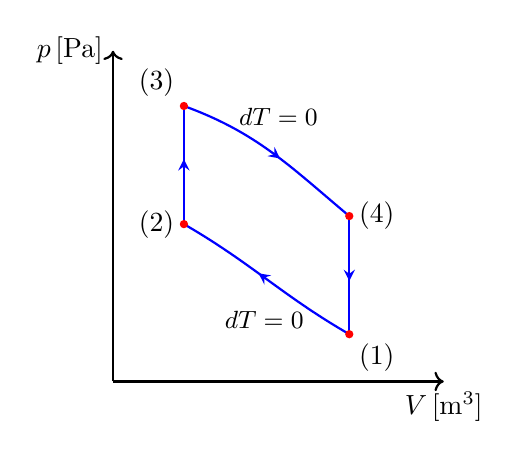
\begin{tikzpicture}[
    % Stílus a vonalak közepén elhelyezett nyilakhoz
    arrow inside/.style={
        postaction={decorate},
        decoration={
            markings,
            mark=at position 0.55 with {\arrow{stealth}}
        }
    }
,scale=0.6]

    % Tengelyek rajzolása feketével, nyilakkal a végén
    \draw[thick, ->] (0,0) -- (7,0) node[below] {$V \, [\mathrm{m^3}]$};
    \draw[thick, ->] (0,0) -- (0,7) node[left] {$p \, [\mathrm{Pa}]$};

    % Pontok koordinátáinak meghatározása
    % Úgy állítjuk be, hogy p3-p2 = p4-p1 legyen (ugyanakkora függőleges szakaszok)
    
    \coordinate (P1) at (5, 1);     % (1) Jobb alsó
    \coordinate (P2) at (1.5, 3.33); % (2) Balra fent (izoterma 1: p*V=5)
    \coordinate (P3) at (1.5, 5.83); % (3) Izochor (p3 = p2 + 2.5)
    \coordinate (P4) at (5, 3.5);    % (4) Izochor (p4 = p1 + 2.5), így p4-p1 = 2.5
    % Megjegyzés: A (3)-(4) görbe így egy másik izoterma (p*V = 1.5*5.83 = 8.75 és 5*3.5 = 17.5)
    % A fizikai hűség kedvéért a (3)-(4) ív is izotermikus marad a rajzon.

    % Folyamatok rajzolása kékkel, középen nyíllal
    % (1) -> (2): Izoterma (dT=0)
    \draw[blue, thick, arrow inside] (P1) to[out=150, in=330] (P2);
    
    % (2) -> (3): Izochor (függőleges, bal oldali)
    \draw[blue, thick, arrow inside] (P2) -- (P3);
    
    % (3) -> (4): Izoterma (dT=0)
    \draw[blue, thick, arrow inside] (P3) to[out=340, in=140] (P4);
    
    % (4) -> (1): Izochor (függőleges, jobb oldali, zárja a kört)
    \draw[blue, thick, arrow inside] (P4) -- (P1);

    % Piros pontok és címkék
    \fill[red] (P1) circle (2.5pt) node[below right, black] {(1)};
    \fill[red] (P2) circle (2.5pt) node[left, black] {(2)};
    \fill[red] (P3) circle (2.5pt) node[above left, black] {(3)};
    \fill[red] (P4) circle (2.5pt) node[right, black] {(4)};

    % Feliratok: dT=0 feketével az izotermák mellett
    \node[black, font=\small] at (3.2, 1.3) {$dT=0$}; 
    \node[black, font=\small] at (3.5, 5.6) {$dT=0$};
\end{tikzpicture}
\end{center}
What is the efficiency of the cycle if $p_{3} = 5 p_{2}$ , the compression ratio is 6, and the cycle is performed with a two-atomic (diatomic) gas? What is the efficiency of the Carnot cycle taking place between the same temperature limits?


\item What is the entropy change if the volume of $ m = 16\,\mathrm{g} $ of oxygen changes from $ V_1 = 20\,\mathrm{l} \text{\ to\ } V_2 = 80\,\mathrm{l},$ and its temperature changes from $t_1 = 90^\circ\mathrm{C} \text{\ to\ } t_2 = 300^\circ\mathrm{C}?$. The molar mass is $ M = 32\,\mathrm{g/mol}.$
  

\end{enumerate}

  
\bigskip

\rightline{Dr.~Gabor~FACSKO}
\rightline{\textit{facsko.gabor@uni-obuda.hu}}

\vfill

\end{document}
